\documentclass{article}
\usepackage[utf8]{inputenc}
\usepackage[dutch]{babel}
\usepackage{amsthm}
\usepackage{hyperref}

\usepackage{graphicx}
\usepackage{subfig}

\title{Project Hartinfarcten}
\author{Arno Deceuninck}


\begin{document}

\maketitle

\tableofcontents

\begin{verbatim}
data <- read.table(file="heart.csv",header=TRUE,sep=";",dec=",")
\end{verbatim}

\subsection{Verwijderde rijen}
Op basis van je studentennummer moesten er enkele rijen verwijderd worden. Dit is gedaan m.b.v. de volgende code in R. 
\begin{verbatim}
# Verwijder de nodige rijen op basis van studienummer s0181217
i <- 2
j <- 1
k <- 7
data <- data[-c(k+1, j+1, i+1, j*k+1, i*j+1, i*k+1, i*j*k+1, i+j+k+1), ]
\end{verbatim}

\section{Verdeling variabele los}

\begin{quote}
\textit{
Bestudeer en bespreek de verdeling van de variabele los. Bespreek hiertoe gepaste grafische
voorstellingen. Ga ook op een formele manier na of de gegevens normaal verdeeld zijn.
Indien dit niet het geval is, in welke zin wijken de gegevens af van normaal verdeelde
gegevens. Kan je de gegevens transformeren naar normaal verdeelde gegevens? Bespreek.}
\end{quote}

\subsection{Normaal verdeeld}
Om een beeld te krijgen van wat de verdeling zou kunnen zijn, heb ik verschillende plots gemaakt hiervan. Op het einde van dit deel wordt er ook formeel getest m.b.v. een shapiro test. We gebruiken hier telkens als teststatistiek de waarden \"los\" uit de meegegeven csv (met de rijen verwijderd zoals hierboven beschreven).  
\begin{verbatim}
los <- data$los
\end{verbatim}
\subsubsection{Boxplot}
\begin{center}
    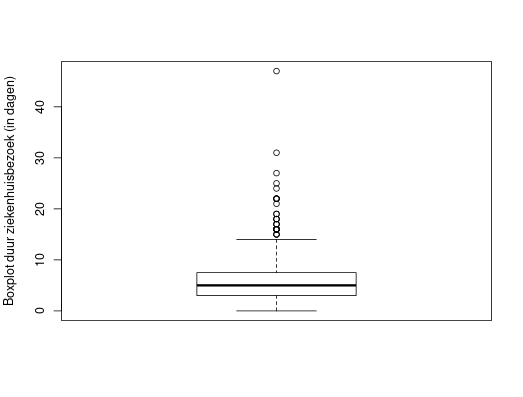
\includegraphics[scale=0.5]{output/boxplot-los.png}
\end{center}
\begin{verbatim}
boxplot(los, ylab="Boxplot duur ziekenhuisbezoek (in dagen)")
\end{verbatim}
Hierin kunnen we al zien dat dit waarschijnlijk geen normale verdeling zal zijn, aangezien er een redelijk lange staart enkel langs rechts is, en dus geen symmetrie.
\subsubsection{Histogram}
\begin{center}
    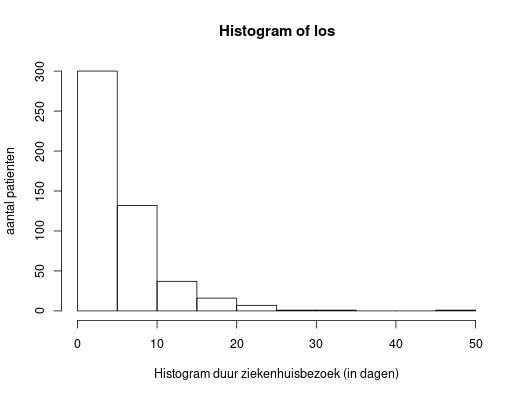
\includegraphics[scale=0.5]{output/Histogram-los.png}
\end{center}

\begin{verbatim}
    hist(los, ylab="aantal patienten", xlab="Histogram duur ziekenhuisbezoek (in dagen)") 
\end{verbatim}
    
Ook hieruit kunnen we afleiden dat er overduidelijk geen symmetrie is en de gegevens dus niet (zonder transformaties) normaal verdeeld kunnen zijn.
\subsubsection{QQ-Plot}
\begin{center}
    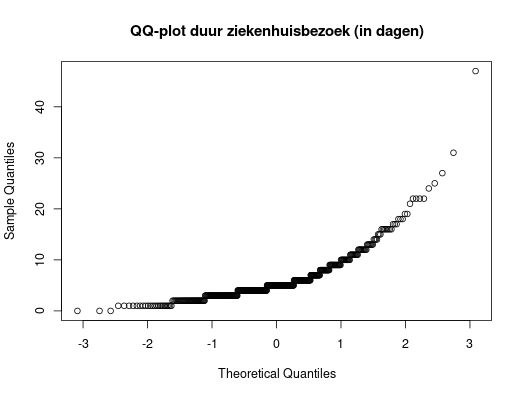
\includegraphics[scale=0.5]{output/qqplot-los.png}
\end{center}
\begin{verbatim}
qqnorm(los, main="QQ-plot duur ziekenhuisbezoek (in dagen)")
\end{verbatim}
Uit deze grafiek kunnen we afleiden welke transformatie we eventueel kunnen doen om een normaalverdeling te krijgen. Om normaal verdeeld te zijn, moet deze grafiek een lineair verband weergeven. We zien echter redelijk duidelijk een exponentieel verband, dus kan het zeker interessant zijn om een kijkje te nemen of het logaritme van je gegevens wel normaal verdeeld is.
\subsubsection{Shapiro test}
We kunnen visueel nu wel besluiten dat de gegevens zonder transformatie niet normaal verdeeld zijn. Dit is echter gewoon op het zicht, dus bij deze doen we ook een formelere test hiervoor, namelijk de Shapiro test. \\ \\
$H_0$: De gegevens van los zijn normaal verdeeld \\
$H_1$: De gegevens van los zijn niet normaal verdeeld 
\begin{verbatim}
shapiro.test(los)
\end{verbatim} 
Deze test geeft als resultaat dat onze p-waarde kleiner is dan 2.2e-16, dus kunnen we inderdaad zegen dat de gegevens van los niet normaal zijn verdeeld.

\subsection{Logaritmisch verdeeld}
We zagen bij het QQ-plot duidelijk dat er een exponentieel verband is, dus nemen we nu een kijkje of het logaritme van die data wel normaal verdeeld is. 

\begin{verbatim}
log_los <- log(los)
\end{verbatim}

Hierbij hebben we echter het probleem dat er mensen tussenzitten die na 0 dagen zijn ontslagen, en $\log(0)$ is geen re\"eel getal (in R is dit $-\inf$), dus halen we de onbepaalde of oneindige gegevens uit onze lijst.

\begin{verbatim}
log_los <- log_los[is.finite(log_los)]
\end{verbatim}

\subsubsection{Grafisch}
We kunnen nu een kijkje nemen of deze getransformeerde gegevens grafisch wel een normaalverdeling vormen.  

\begin{figure}[!htb]
\minipage{0.32\textwidth}
  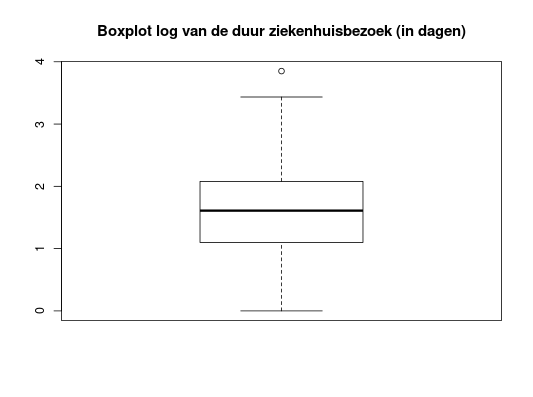
\includegraphics[width=\linewidth]{output/boxplot-loglos.png}
\endminipage\hfill
\minipage{0.32\textwidth}
  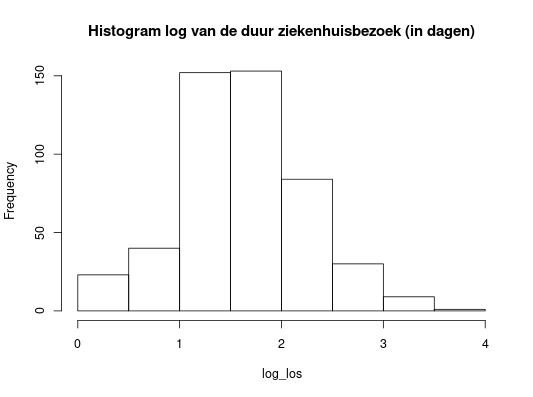
\includegraphics[width=\linewidth]{output/histogram-loglos.png}
\endminipage\hfill
\minipage{0.32\textwidth}%
  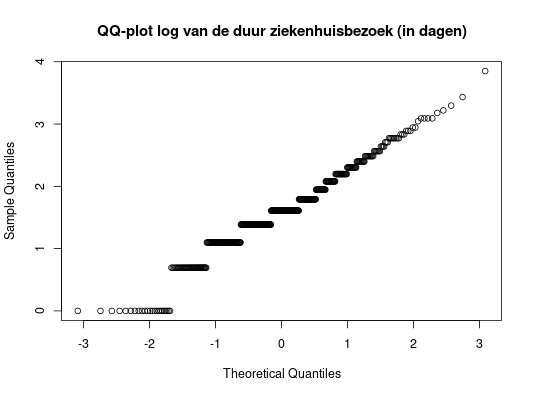
\includegraphics[width=\linewidth]{output/qqplot-loglos.png}
\endminipage
\end{figure}

\begin{verbatim}
qqnorm(log_los, main="QQ-plot log van de duur ziekenhuisbezoek (in dagen)")
boxplot(log_los, main="Boxplot log van de duur ziekenhuisbezoek (in dagen)")
hist(log_los, main="Histogram log van de duur ziekenhuisbezoek (in dagen)")
\end{verbatim}
Hier kunnen we wel al de kenmerken van een normaalverdeling in terugvinden. Vooral het QQ-Plot is opvallend: we kunnen hier duidelijk een lineair verband in terugvinden, wat dus zou wijzen op een normaalverdeling. Bij het QQ-Plot is het echter opvallend dat het aantal dagen een discrete veranderlijke is, wat een normale verdeling sowieso onmogelijk maakt. 

\subsubsection{Shapiro test}

We zullen nog formeel testen dat dit geen normaal verdeling is (door het discreet zijn) a.d.h.v. een Shapiro test.  \\ \\
$H_0$: De gegevens van los zijn normaal verdeeld \\
$H_1$: De gegevens van los zijn niet normaal verdeeld 
\begin{verbatim}
shapiro.test(log_los)
\end{verbatim}

Dit geeft als p-waarde 1.197e-07, wat nogsteeds te klein is, dus we verwerpen onze $H_0$. Het is dus niet normaal verdeeld. 

\subsection{Conclusie}
We konden dus duidelijk een langere staart zien langs rechts bij zowel het boxplot als het histogram. Het QQ-plot liet duidelijk zien dat de gegevens niet normaal verdeeld waren en gaf het idee om het logaritme van de gegevens te nemen. Dit kwam heel sterk in de buurt van een normale verdeling. In het QQ-plot kon je wel een rechte herkennen, maar deze was opgesplitst in treden omdat het aantal dagen een discrete veranderlijke was. De Shapiro test verwierp dus ook dit resultaat. We kunnen niet a.d.h.v. een transformatie het discrete continu maken. Het logaritme nemen blijft dus de transformatie die ons het dichste bij de normale verdeling brengt.

\section{Verband duur, dood/levend}

\begin{quote}
\textit{
Hangt de duur van het ziekenhuisverblijf af van het levend of gestorven zijn van de
patiënten? M.a.w. is de duur van het ziekenhuisverblijf identiek verdeeld bij de populatie levende en gestorven patiënten? Voer een gepaste test uit.}
\end{quote}

\subsection{Opmerking}
Het was niet direct duidelijk over wanneer het "levend of gestorven zijn" ging, na de laatste opvolging of op het moment van het ontslag uit het ziekenhuis. Ik ben ervan uit gegaan dat het om de laatste opvolging ging.

\subsection{Teststatistiek}
Hierbij heb ik gebruik gemaakt van de variabele fstat en los uit de data uit de csv (met de nodige rijen eruit gehaald).

\begin{verbatim}
alive <- data$los[data$fstat=="0"] # Patienten levend bij laatste opvolging
dead <- data$los[data$fstat=="1"] # Patienten dood bij laatste opvolging
\end{verbatim} 

\subsection{Test}
Om een t-test uit te voeren moet ik eerst nagaan of de variantie voor beide groepen gelijk zijn. \\ \\
$H_0$: Beide groepen hebben dezelfde variantie. \\
$H_1$: De variantie van de groepen is verschillend. 

\begin{verbatim}
var.test(alive, dead)
\end{verbatim}

Als resultaat van deze test krijg ik als p-waarde 0.6906. Dit is duidelijk groter dan 0.05, dus we kunnen er vanuit gaan dat de variantie voor beide groepen hetzelfde is (we aanvaarden $H_0$ en dus verliezen we hierdoor geen vrijheidsgraad).

We kunnen nu dus onze t-test zelf uitvoeren met gelijke variantie. \\ \\
$H_0$: Er is geen verschil tussen beide verdelingen. \\
$H_1$: Er is wel een verschil. 

\begin{verbatim}
t.test(dead, alive, var.equal=TRUE)
\end{verbatim}

Dit geeft als p-waarde 0.08156, wat dus betekent dat we onze $H_0$ kunnen behouden: De twee variabelen hangen dus niet af van elkaar. 

\section{Verband type hartinfarct/ontslagstatus}
\begin{quote}
\textit{
Ga na of er een verband is tussen het type hartinfarct en de ontslagstatus uit het ziekenhuis
na opname. Voer opnieuw een gepaste test uit.}
\end{quote}

\subsection{Type test}
We zitten met groepen, dus discrete variabelen. Een $\chi^2$-test is hier van toepassing. Als teststatistiek gebruiken we de waarden dstat en mitype uit de data. 

\begin{verbatim}
dstat <- data$dstat
mitype <- data$mitype
\end{verbatim}

\subsection{Test}
We beginnen met een contingentietabel op te stellen. We beginnen met op de rijen te zetten of de patienten levend of dood waren bij ontslag en op de kolom het type hartinfectie. 

\begin{verbatim}
alive <- c(nrow(data[dstat=="0" & mitype=="0",]), nrow(data[dstat=="0" & mitype=="1",]))
dead <- c(nrow(data[dstat=="1" & mitype=="0",]), nrow(data[dstat=="1" & mitype=="1",]))
ctable <- data.frame(alive, dead)
\end{verbatim}

Hieruit berekenen we enkele waarden m.b.v. een $\chi^2$-test. De gegevens ervan zetten we hieronder op een rijtje. \\ \\
$H_0$: Het type hartinfarct en ontslagstatus uit het ziekenhuis zijn onafhankelijk van elkaar.\\
$H_1$: Deze twee zijn wel afhankelijk van elkaar.

\begin{verbatim}
chiSq <- chisq.test(ctable)
\end{verbatim}

\begin{table}[h]
%\centering
\begin{tabular}{|l|l|l|}
\hline
       & geen Q-golven & wel Q-golven \\ \hline
levend & 318           & 138          \\ \hline
dood   & 28            & 11           \\ \hline
\end{tabular}
\quad
%\begin{table}[]
%\centering
\begin{tabular}{|l|l|l|}
\hline
       & geen Q-golven & wel Q-golven \\ \hline
levend & 318.7394      & 137.2606     \\ \hline
dood   & 27.26061      & 11.73939     \\ \hline
\end{tabular}
\caption{links: geobserveerde waarden, rechts: verwachte waarden}
\end{table}

\begin{table}[h]
\centering
\begin{tabular}{|l|l|l|}
\hline
$\chi^2$  & df & p-waarde \\ \hline
0.0075814 & 1  & 0.9306   \\ \hline
\end{tabular}
\caption{resultaat test}
\end{table}

De test is ook gedaan met rijen en kolommen omgewisseld en dit gaf, zoals verwacht, dezelfde resultaten. Onze p-waarde is groter dan 0.05, dus we kunnen $H_0$ aanvaarden: er is geen verband tussen de twee. 

\section{Leeftijd voorspellen uit BMI}
\subsection{Teststatistiek}
Als teststatistiek worden de kolommen age en bmi uit de data gebruikt. Om het type test te berekenen moeten we eerst zien of deze gegevens normaal verdeeld zijn. 

\begin{verbatim}
qqnorm(data$age, main = "Normaalverdeling leeftijd")
qqnorm(data$bmi, main = "Normaalverdeling BMI")
\end{verbatim}

\begin{figure}[h]%
    \centering
    \subfloat[QQ-Plot leeftijd]{{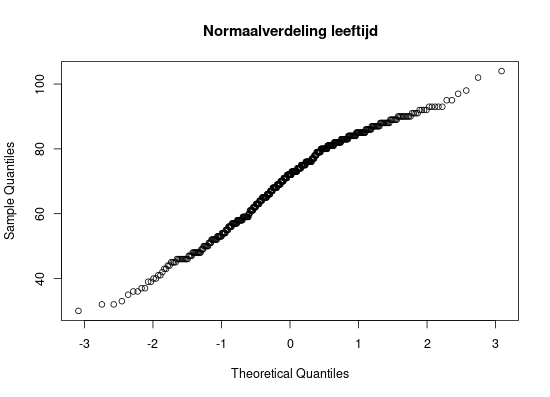
\includegraphics[width=5cm]{output/normaal-age.png} }}%
    \qquad
    \subfloat[QQ-Plot BMI]{{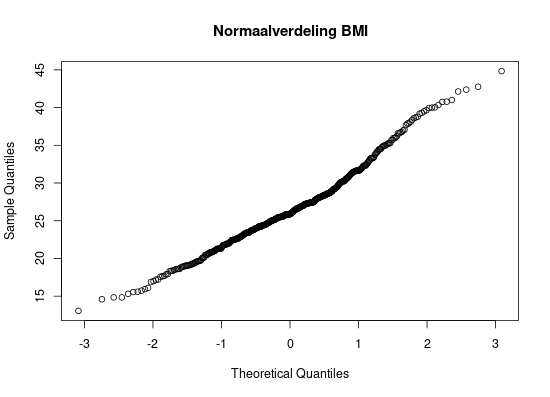
\includegraphics[width=5cm]{output/normaal-bmi.png} }}%
\end{figure}

We kunnen in beide gevallen wel een lineair verband herkennen, maar doen toch een shapiro test om er zeker van te zijn. \\ \\
$H_0$: BMI en leeftijd zijn normaal verdeeld.\\
$H_1$: Ze zijn niet normaal verdeeld.

\begin{verbatim}
shapiro.test(data$age)
shapiro.test(data$bmi)
\end{verbatim} 

Beide tests geven een te kleine p-waarde ($H_0$ wordt verwerpt), dus kunnen we er niet vanuit gaan dat deze normaal verdeeld zijn. Pearsons correlatiecoefficient kunnen we dus niet gebruiken, dus gebruik ik Spearman's test in de plaats.

\begin{center}
    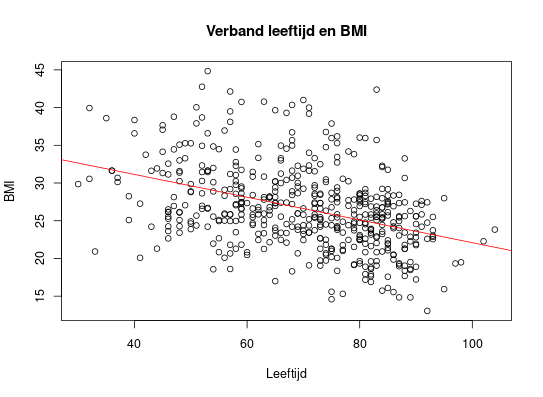
\includegraphics[scale=0.5]{output/linreg-scatter.png}
\end{center}

\begin{verbatim}
plot(data$age, data$bmi, type="p", xlab="Leeftijd", ylab="BMI", 
	     main="Verband leeftijd en BMI")
abline(linreg,col="red",lty=1)
\end{verbatim}

\subsection{Spearman's test}
$H_0$ : er is geen monotoon verband tussen leeftijd en BMI
$H_1$ : er is een mate van monotoon verband tussen leeftijd en BMI

\begin{verbatim}
cor.test(data$age, data$bmi, method = "spearman") 
\end{verbatim}

We merken dat onze p-waarde hier veel te klein is, dus moeten we $H_0$ verwerpen: Er is een mate van monotoon verband tussen leeftijd en BMI. De Spearman correlatieco\"effici\"ent is negatief, wat erop wijst dat de ene variabele stijgt terwijl de andere afneemt.

\subsection{Lineaire regressie}

We zullen nu m.b.v. lineaire regressie onderzoeken of het zinvol is om te stellen dat dit verband lineair is. \\ \\

$H_0$ : er is een lineair verband tussen leeftijd en bmi\\
$H_1$ : er is geen lineair verband tussen de twee

\begin{verbatim}
linreg <- lm(data$bmi ~ data$age)
summary(linreg)
\end{verbatim}

Dit geeft ons \^a = 37.16551 en \^b = -0.15081. De regressierechte wordt dus: BMI = 37.16551 - 0.15081 * leeftijd. $R^2$ is 0.1608, wat inhoudt dat slechts 16.08\% van de variabiliteit op het BMI verklaard wordt door de leeftijd. Onze p-waarde (van de F-test) is onder 0.05, wat wil zeggen dat het model niet zinvol is. We kunnen het BMI dus niet voorspellen uit de leeftijd.

%We zullen nog nagaan of de fouttermen normaal verdeeld zijn.
%
%\begin{verbatim}
%res <- residuals(linreg)
%qqnorm(res,xlab="Standard Normal Quantiles",
%ylab="Raw Residuals",main="Raw Residual-Normal QQ-plot")
%\end{verbatim}
%
%\begin{center}
%    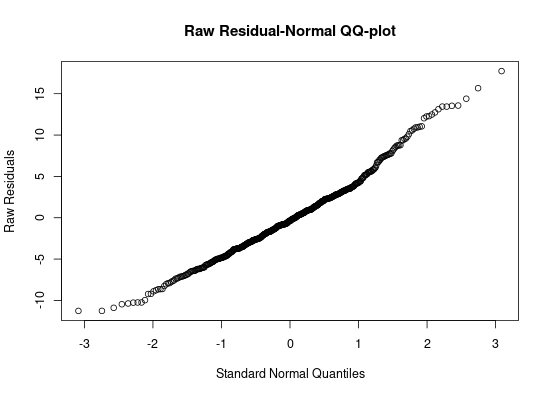
\includegraphics[scale=0.5]{output/residual.png}
%\end{center}
%
%\begin{figure}[!htb]
%\minipage{0.32\textwidth}
%  \includegraphics[width=\linewidth]{output/%linreg-scatter.png}
%\endminipage\hfill
%\minipage{0.32\textwidth}
%  \includegraphics[width=\linewidth]{output/%stand-res.png}
%\endminipage\hfill
%\minipage{0.32\textwidth}%
%  \includegraphics[width=\linewidth]{output/pred-%bmi.png}
%\endminipage
%\end{figure}




\end{document}
